\chapter{System Implementation And Experimental Evaluation} \label{chap:system_implementation}
    This chapter attempts to discusses the experiments performed to evaluate the proposed solutions as well as the tools that were utilized for the implementation of the system. Section \ref{sec:experimental_setup} provides information about the system design, choice of software and programming languages that were utilized to develop the system. Section \ref{sec:evaluation_of_snapshot_materialization} provides an evaluation of discussed methods for snapshot materialization by setting up different experiments. In section \ref{}, different malicious activity scenarios on the relational database are introduced and the Blockchain solution to identify these activities is discussed.

	\section{Development environment and application development tools} \label{sec:development environment}
		To setup the development environment of the project, we used the 'Leda' research server provided by the department of scinece at the University of Ontario Institute of Technology with the ubuntu 16.04 operating system installed. The application could be developed by various tools, but since one important goal of this project was to be able to generalize our proposed solution for different systems, we needed to choose the tools that are popular among the developers for the development of their system. For the database choice, we favored the use of postgreSQL simply because of its wide adoptation by the industry \cite{cook2017docker}. 

		The experiments scripts were mainly developed by using Python 2.7 programming language. We started off by generating database using the TPCH schema with 1,000,000 tuples in the main table. We also generated a synthetic temporal database by performing a set of random record modification, insertion and deletion updates at 1000 distinct timestamps. This created a temporal table with 1,000 timestamps. To be able to manage the relational database and perform queries on the tables, we utilized SQL query language.

		Generation of snapshots using the records stored in the temporal tables required time series analysis and performing numbers of aggregations and self-joins on the table. In order to make this process more efficient and less cumbersome, we utilized the windowing function that is part of the SQL standard and is supported by the relational databases \cite{leis2015efficient}.

		To evaluate the effectiveness of snapshot materialization, the optimal snapshot placement had to be examined in different query distributions on the timeline. The Python's Numpy library gave us the ability to simulate some hotspots on the timeline and distribute the queries on the timeline with various distribution models. After running the snapshot materialization experiments and collecting data, we utilized the Python's plotly library in order to visualize the collected data.

		Cryptography is the method that Blockchain utilizes to secure data that are stored in it and link the blocks of data together. For the purpose of creating a Blockchain of the records, we used the Python's pycrypto 2.6.1 library \footnote{https://pypi.org/project/pycrypto/}. The pycripto package contains various encryption algorithms and hash functions as well as a built-in function to create digital signatures that makes it suitable for the creation of the Blockchain.

	\section{Evaluating snapshot materialization} \label{sec:evaluation_of_snapshot_materialization}
		In this section we discuss the evaluation of snapshot materialization through different experiments. We start off by showing a method to create snapshots using the data that are stored in the temporal database. Then we show the problem of linear computational time in performing queries on a temporal relational table and we evaluate the placement of a single snapshot for matrialization in different timestamps. In the next step we show the effectiveness of utilizing multiple number of precomputed snapshots for materialization and at the end, the various approaches discussed in section \ref{sec:optimal_multiple_snapshot} to place multiple snapshots on the timeline are put to an experiment and their performance is evaluated.

		\subsection {Generating snapshots by using records in a temporal database} \label{sec:snapshot_generation}
			We can construct the snapshots using simple windowing functions (as in supported by PostgreSQL \cite{momjian2001postgresql}).
    		\vspace{1em}
			\begin{center}
				\begin{table}[b]
					\centering
					\small
						\begin{tabular}{|l|} \hline
							$\mathrm{snapshot}(r, t)$ = \\
							\verb|| \textsc{With} $T$ \textsc{as} ( \\
							\verb|   | \textsc{select} id, $\{\mathrm{last\_value}(x) \mathrm{\ as\ } x:
							x\in attr(r)\}$ \textsc{over} $W$ \\
							\verb|   | \textsc{from} $r^T$ \\
							\verb|   | \textsc{where} updates $\leq t$ \\
							\verb|   | \textsc{window} $W$ \textsc{as} 
							\textsc{partition by} id \textsc{order by} updates\\
							\verb|| ) \\
							\verb|| \textsc{select} id, $\{x: x\in attr(r)\}$ \textsc{from} $T$ \\
							\verb|| \textsc{where not} $T.$deleted \\ \hline
						\end{tabular}
					
				\end{table}
			\end{center}
			The query $\mathrm{snapshot}(r, t)$ computes the snapshot of $r$ at timestamp $t$ by applying the latest update of each tuple up to timestamp $t$, while removing tuples that have been deleted.

		\subsection{Evaluating the linearity of the queries on a temporal table} \label{sec:evaluating_linearity}
			As discussed in proposition \ref{prop:linear_time}, preforming queires to create snapshots in a timestamp of interest from the historical data, require visiting all the records before that timestamp and apply all the updates on the table. Over time, when the temporal tables grow in size, performing such computations may become expensive and inefficient. To prove it experimentally, we implemented a function to perform snapshot creation query on our temporal table and record the query runtime. Then we performed this query 100 times while sliding the timestamp of the query on the timeline of the temporal table. By sliding the timestamp, in each iteration of the query, more records needed to be visited and more updates needed to be applied. From the runtime records the costline was created which is shown if Figure \ref{fig:linear_time}. 

			Figure \ref{fig:linear_time} clearly proves our claim that computation of snapshots on a temporal table requires linear time. The issue of linearity in computation of snapshots makes such tasks on a very large table inefficient. For example in this experiment, the computational cost of 100th query is significantly more expensive than computational cost of 20th query, due to the number of queries which were needed to be visited.

			\begin{figure}
				\centering
				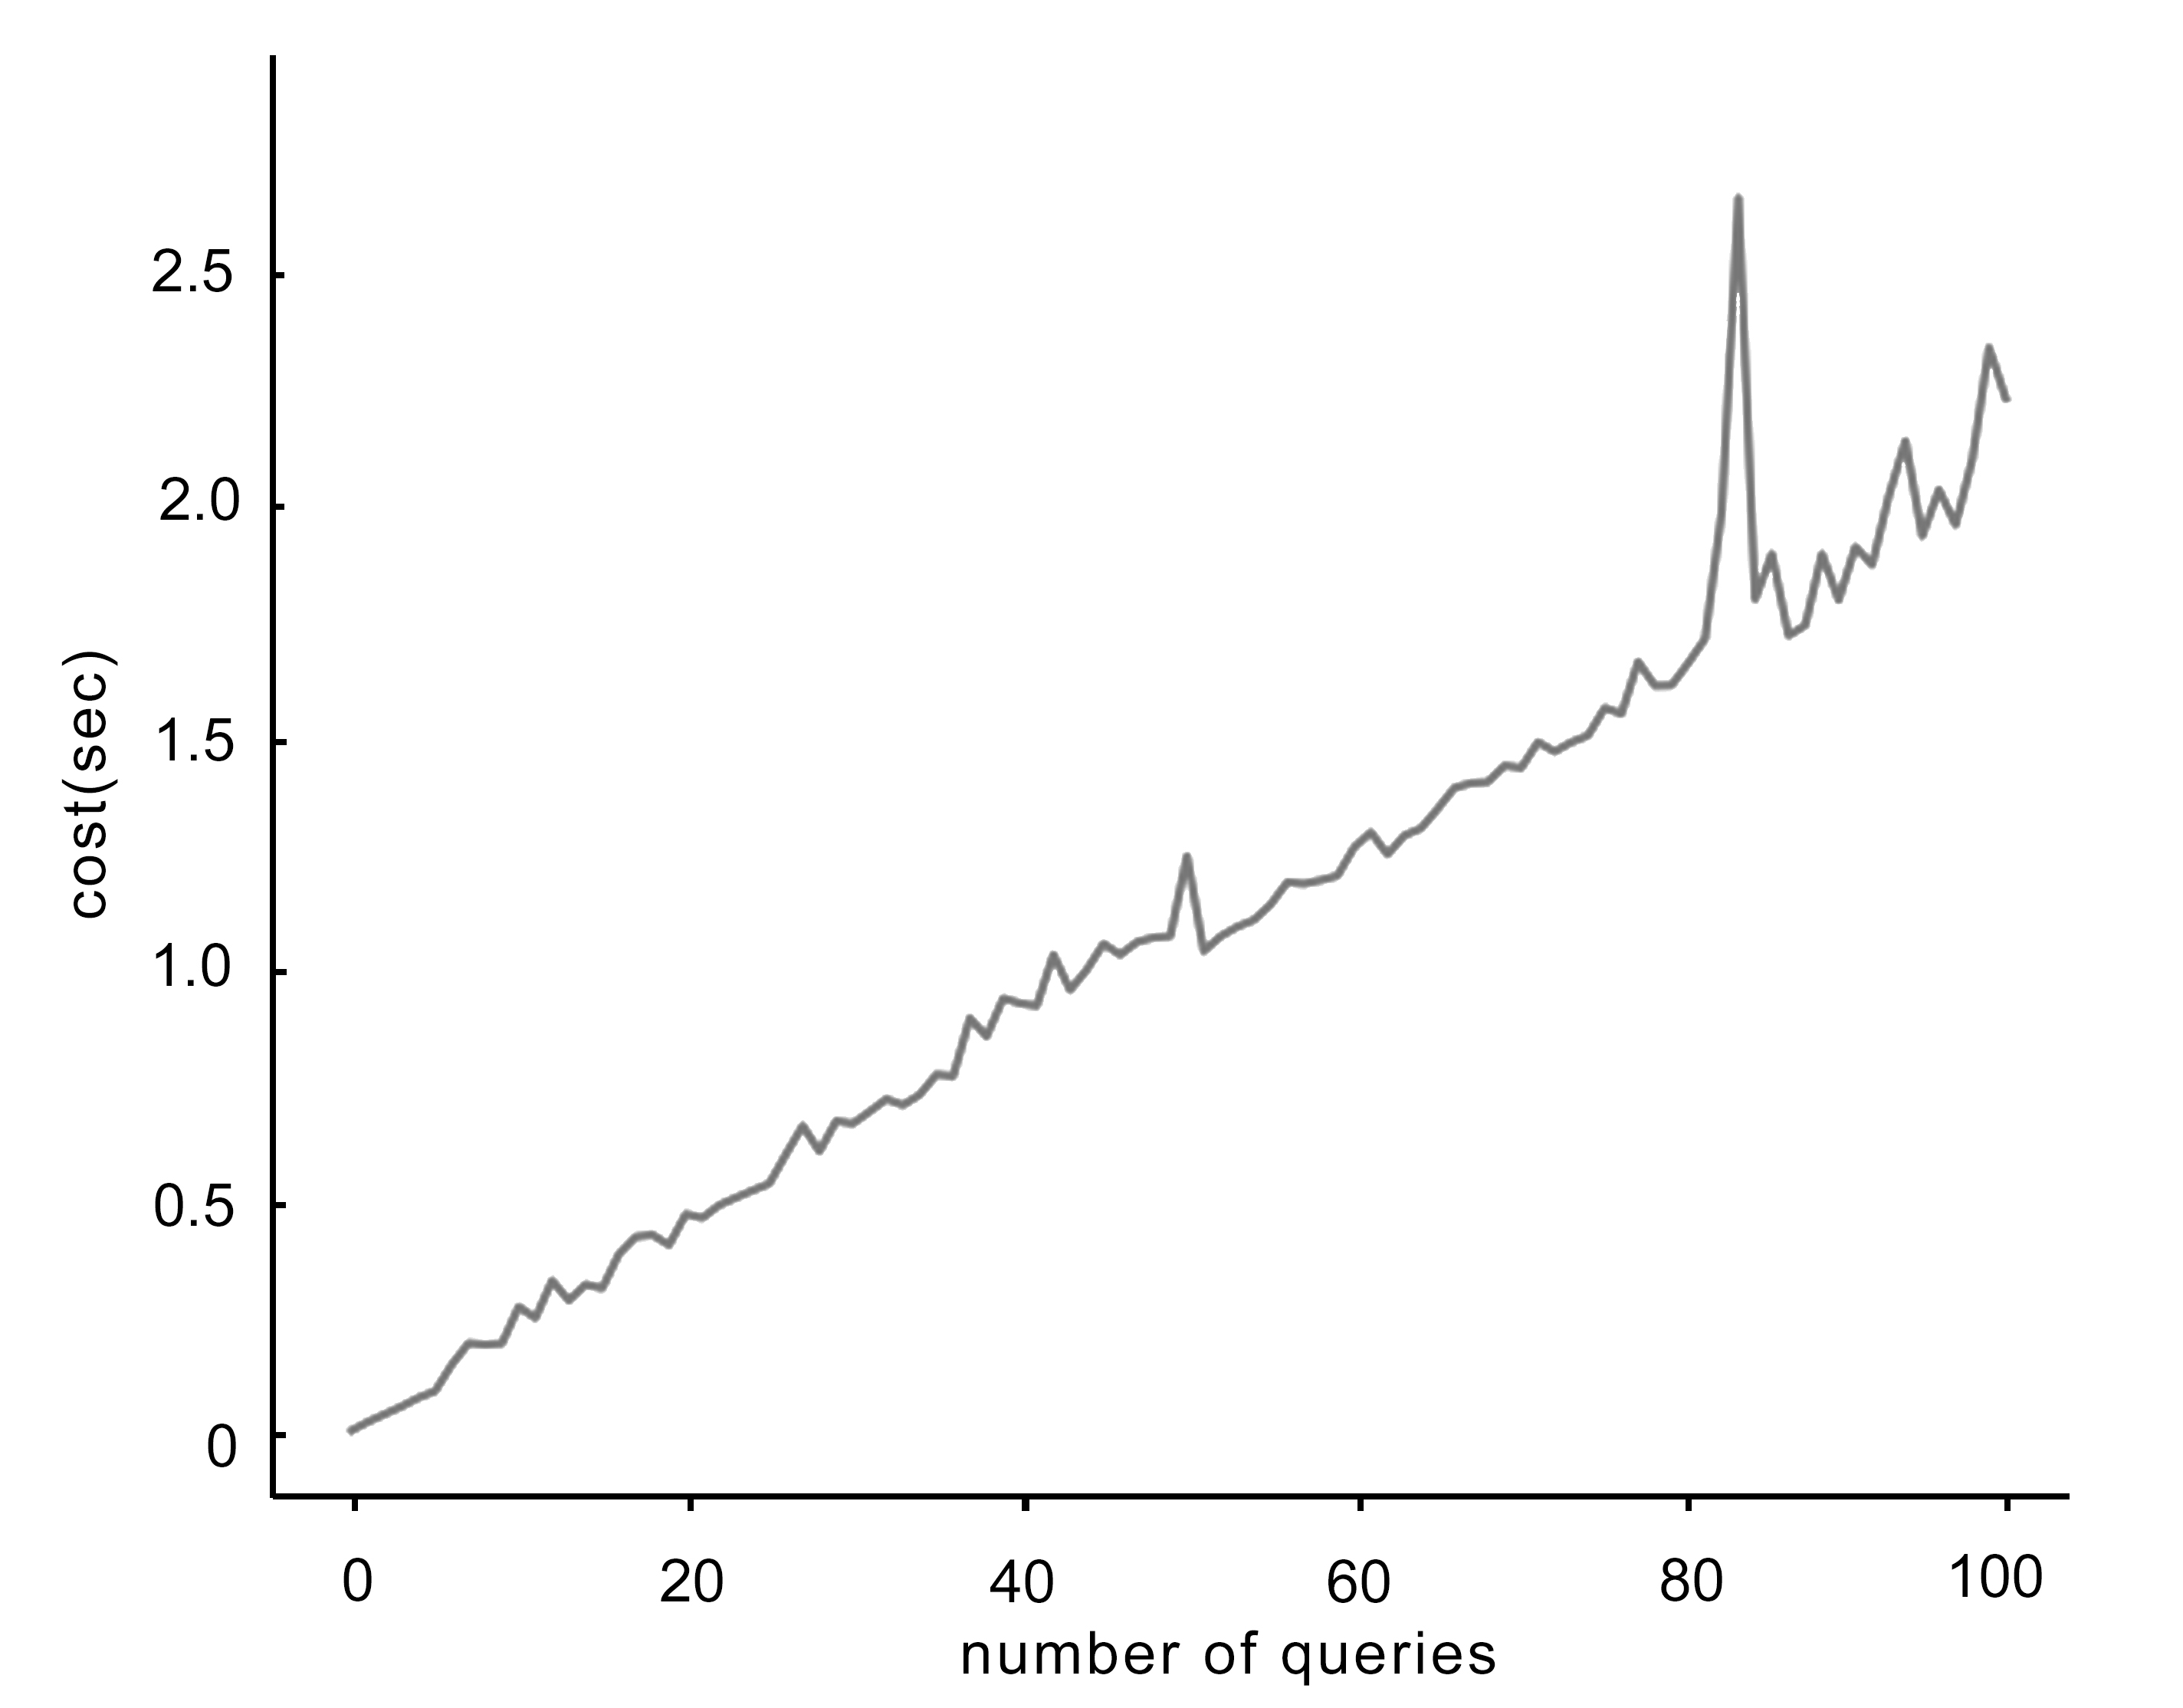
\includegraphics[width=120mm]{figs/runtime.jpg}
				\caption{Linear time in computation of snapshots without snapshot materialization}
				\label{fig:linear_time}
			\end{figure} 

		\subsection{Evaluating materialization of a single snapshot} \label{sec:evaluating_single_snapshot}
			To illusterate the the optimal position on the timeline to place a single snapshot for materialization, we sampled 60 query timestamps from our temporal database and randomly placed 60 number of queries on its timeline. In the next step we placed a single snapshot that each query materialized to perform the task and recorded the overal cost of queries on that timeline using definition \ref{defn:cost_of_query_answering}. To see how the position of materialized snapshot may affect the overal cost of query answering, we slided the timestamp of the snashot on the timeline and recorded the overal cost in each snapshot timestamp. The resulted cost line obtained from sliding the snapshot is depicted in Figure \ref{fig:single_snapshot}. 

			The resulted cost line shown in Figure \ref{fig:single_snapshot} clearly shows that the position of a snapshot directly affects the overal cost of query answering on the temporal table. In proposition \ref{prop:compute-median} we mathematically proved that the median of the queries is the optimal position for snapshot materialization. Therefore in this experiment we calculated the median of the queries which is shown with a red circle in figure \ref{fig:single_snapshot}. As it could be seen, the median of the queries is exactly located in a position where the cost line curve's global minimum is. This illustrates that the median of the queries is the most optimal position to place a single snapshot for materialization.

			\begin{figure}
				\centering
				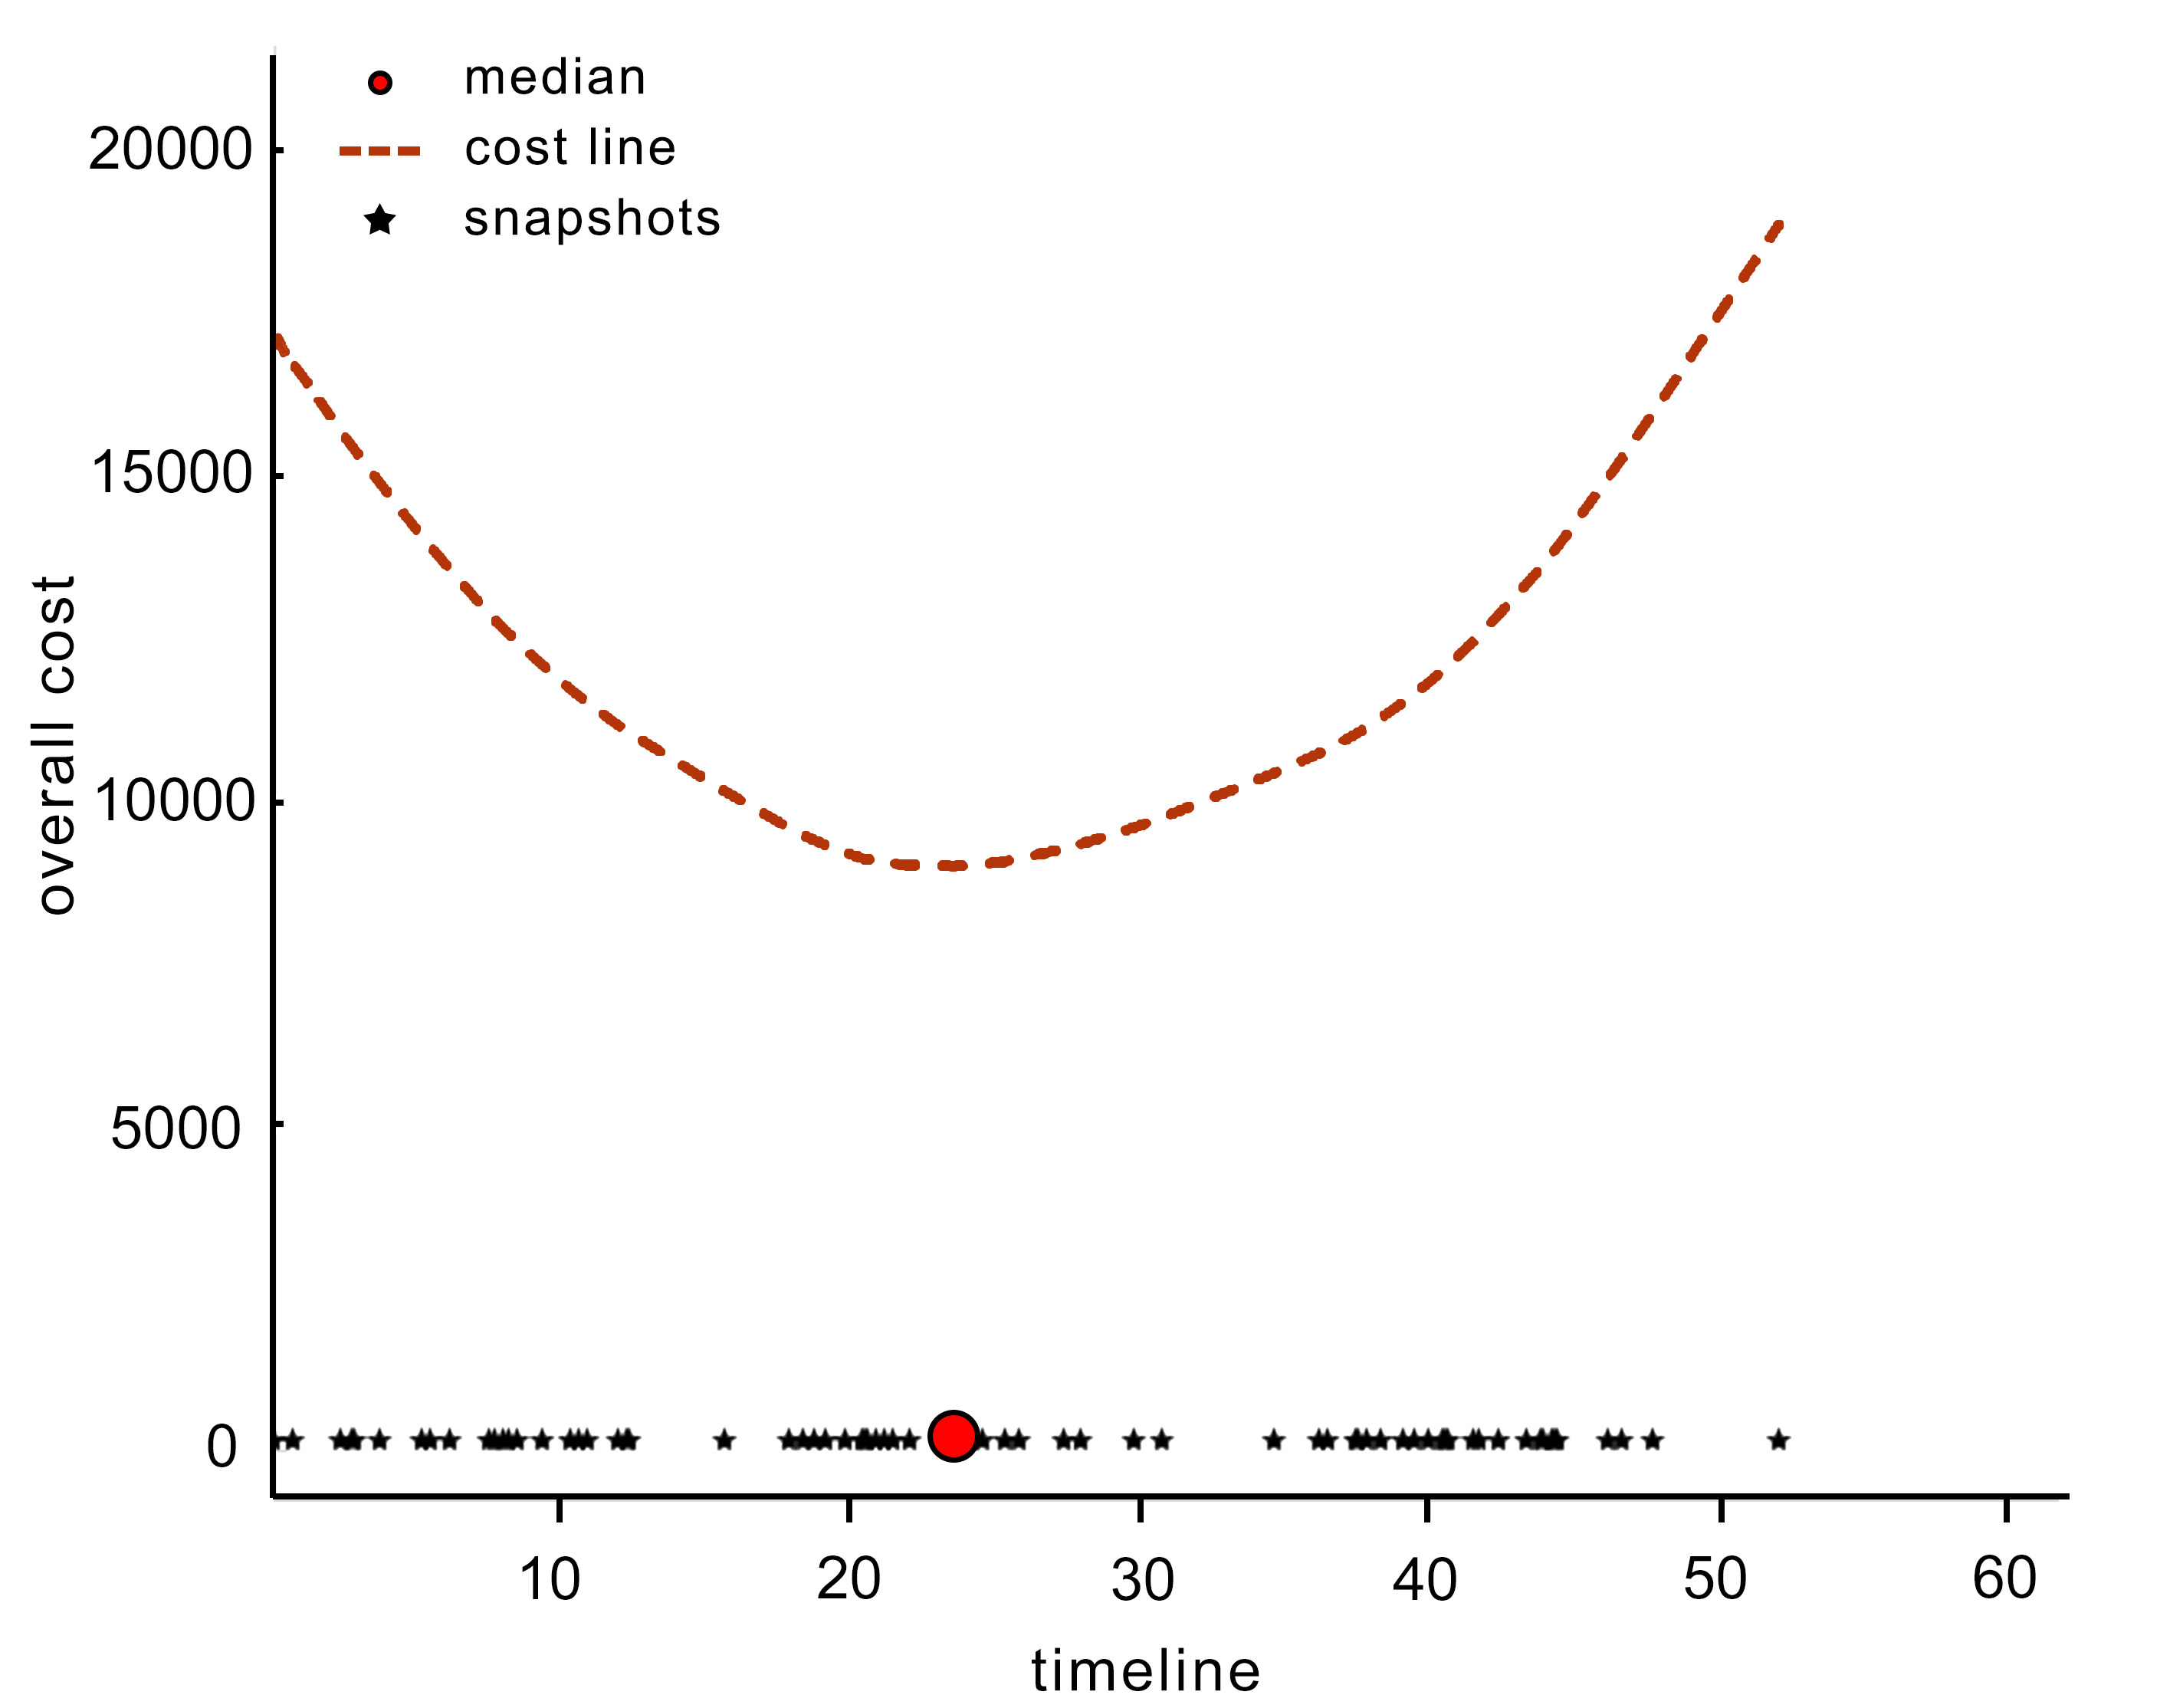
\includegraphics[width=90mm]{figs/single_snapshot.jpg}
				\caption{Cost of query answering using a single snapshot over different snaptshot timestamps}
				\label{fig:single_snapshot}
			\end{figure} 

		\subsection{Evaluating materialization of multiple snapshot} \label{evaluating_multiple_snapshots}
			To evaluate the performance of our optimal snapshot computation, we evaluated the recursive formulation given
			by Section \ref{}, the dynamic programming formulation given by Section \ref{} and heuristic method given by Section \ref{}. 

			To illustrate that the optimal snapshot placement indeed produces the best query answering performance, we compared the query answering cost of three approaches:
			\begin{itemize}
				\item Pick $m$ random timestamps to place the snapshots.
				\item Pick $m$ evenly intervaled timestamps to place the snapshots.
				\item Pick $m$ timestamps computed by dynamic programming.
			\end{itemize}

			\begin{figure}
				\centering
				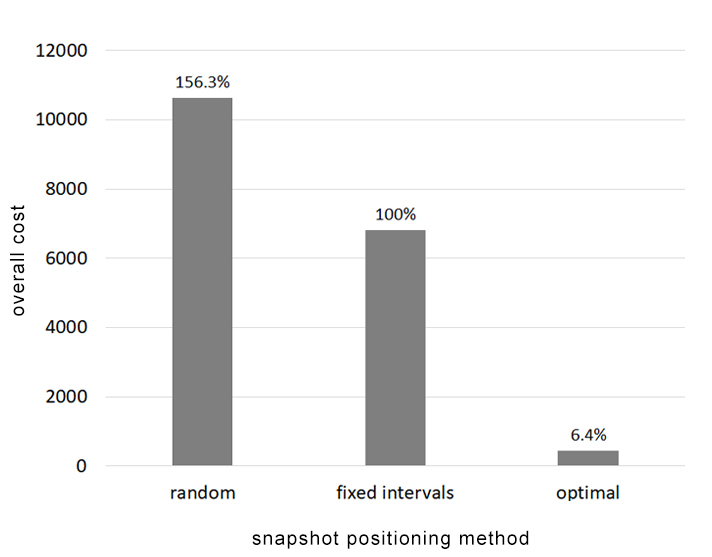
\includegraphics[width=80mm]{figs/various_scenarios_cost.jpg}
				\caption{Query answering cost with forty snapshots with various approaches to place snapshots for materialization}
				\label{fig:approaches_cost}
			\end{figure} 

			Figure \ref{fig:approaches_cost} shows that the placements obtained by dynamic programming clearly beats the other two approaches.

			In order to evaluate the effectiveness of $m$ number of snapshots to lower the overal cost of query answering, we recorded the overal cost of queries in various number of snapshots. Figure \ref{fig:snapshots_cost} shows that as the number of snapshots for materialization increases, the overal cost of answering to the queries drops.

			\begin{figure}
				\centering
				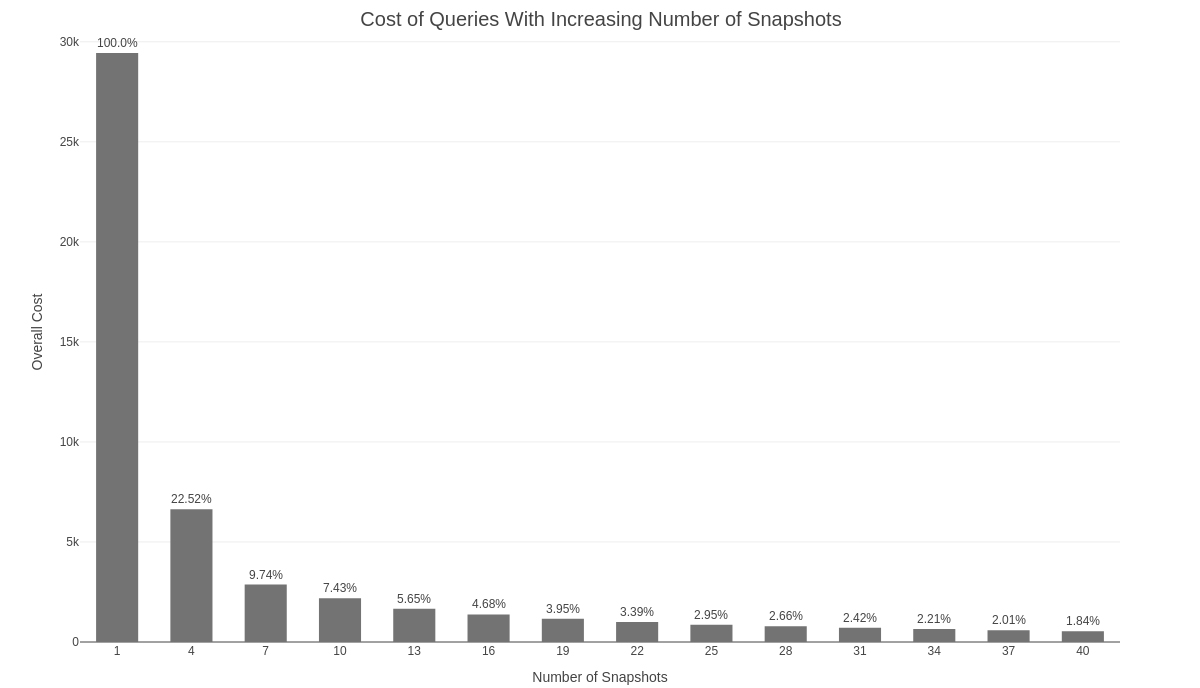
\includegraphics[width=\textwidth]{figs/various_snapshot.jpg}
				\caption{Query answering cost with increasing number of snapshots}
				\label{fig:snapshots_cost}
			\end{figure} 

		\subsection{Implementation of recursive algorithm} \label{sec:recursive_implementation}
			Recursive method was our first approach to find $m$ number of optimal segmentations of the timeline for snapshot placement. The recursive algorithm of this operation is given as Algorithm \ref{alg:recursive}.

			\begin{algorithm}
				\SetAlgoLined
				\caption{Dynamic programming method to compute $m$ number of optimal segmentations}
				\SetAlCapNameFnt{\tiny}
				\label{alg:recursive}
				\DontPrintSemicolon
				 \SetKwFunction{FMain}{computeOPT}
				 \SetKwProg{Fn}{Function}{:}{}
				 \Fn{\FMain{$Q$, $m$}}{
				    $n = |Q|$\;
				    \textbf{OPT}$[i,0]$ = $\infty$ \;
				    \For{$k \gets 1$ \KwTo $m$}{
				    	\For{$i \gets 1$ \KwTo $n$}{
				    		$j^* = \underset{j\in[1,i]}{\mathrm{argmin}}(\mathrm{cost}(\mathbf{OPT}[j,k-1]) + \mathrm{cost}(Q[j+1, n]))$ \;
				    		$\mathbf{OPT}[i,k] = \mathbf{OPT}[j^*, k-1] \cup \{\mathrm{median}(Q[j+1], n)\}$ 
				    	}
				    }
				}
			\end{algorithm}

		\subsection{Implementation of dynamic programming} \label{sec:dynamic_implementation}
			Dynamic programming was the second approach that we utilized in order to find $m$ number of optimal segmentation of the timeline for snapshot placement. This approach could be implemented using Algorithm \ref{alg:dynamic_programming}.
			\begin{algorithm}
				\SetAlgoLined
				\caption{Dynamic programming method to compute $m$ number of optimal segmentations}
				\SetAlCapNameFnt{\tiny}
				\label{alg:dynamic_programming}
				\DontPrintSemicolon
				 \SetKwFunction{FMain}{computeOPT}
				 \SetKwProg{Fn}{Function}{:}{}
				 \Fn{\FMain{$Q$, $m$}}{
				    $n = |Q|$\;
				    \textbf{OPT}$[i,0]$ = $\infty$ \;
				    \For{$k \gets 1$ \KwTo $m$}{
				    	\For{$i \gets 1$ \KwTo $n$}{
				    		$j^* = \underset{j\in[1,i]}{\mathrm{argmin}}(\mathrm{cost}(\mathbf{OPT}[j,k-1]) + \mathrm{cost}(Q[j+1, n]))$ \;
				    		$\mathbf{OPT}[i,k] = \mathbf{OPT}[j^*, k-1] \cup \{\mathrm{median}(Q[j+1], n)\}$ 
				    	}
				    }
				}
			\end{algorithm}

		\subsection{Implementation of heuristic method} \label{sec:implementation_heuristic}
			To evaluate the performance of heuristic method in finding $m$ number of optimal segmentation of the timeline for snapshot placement, we chose K-means clustering method. The K-means clustering algorithm is given as Algorithm \ref{alg:Kmeans}.
			\begin{algorithm}[H]
				\SetAlgoLined
				\caption{K-means clustering to compute $m$ number of segmentations}
				\label{alg:Kmeans}
				\DontPrintSemicolon
				 \SetKwFunction{FMain}{K-Means}
				 \SetKwProg{Fn}{Function}{:}{}
				 \Fn{\FMain{$T_q^*\{q_1,...,q_n\}$, $m$}}{
				    $\{\mu_1,...,\mu_m\} \gets SelectRandomSeeds(\{q_i\in T_q^*\},m)$ \;
					\For{$i \gets 1$ \KwTo $n$}{
						$J \gets argmin_{J^*}||\mu_{J^*}-q_i||^2$ \;
						$\mathcal{L}_j \gets \mathcal{L}_j \cup \{q_i\}$ 
					}
					\For{$j \gets 1$ \KwTo $m$}{
						$\mu_j \gets \frac{1}{\mathcal{L}_j} \sum_{q \in \mathcal{L}_j} q $
					}
					\Return\{$\mu_1,...,\mu_m$\}
				}
			\end{algorithm}

		\subsection{Evaluating approaches for optimal placement of $m$ snapshots} \label{sec:evaluating_approaches}
			As discussed in section \ref{}, we examine 3 approaches to find the optimal timestamps for $m$ number of snashots for materialization. The performed approaches are:
			\begin{itemize}
				\item Recursive algorithm.
				\item Dynamic programming.
				\item K-Means clustering.
			\end{itemize}

			In the first experiment of this category, we evaluate the performance of each approach with respect to variable number of snapshots but fixed number of queries. That is, although the goal of the experiment is to find $m$ number of optimal timestamps for snapshots for materialization, but we start $m=1$ and we increase $m$ in each iteration. For this experiment we sampled 140 number of queries and evalueted the runtime of each approach while increasing the number of requested snapshots.

			\begin{figure}
				\centering
				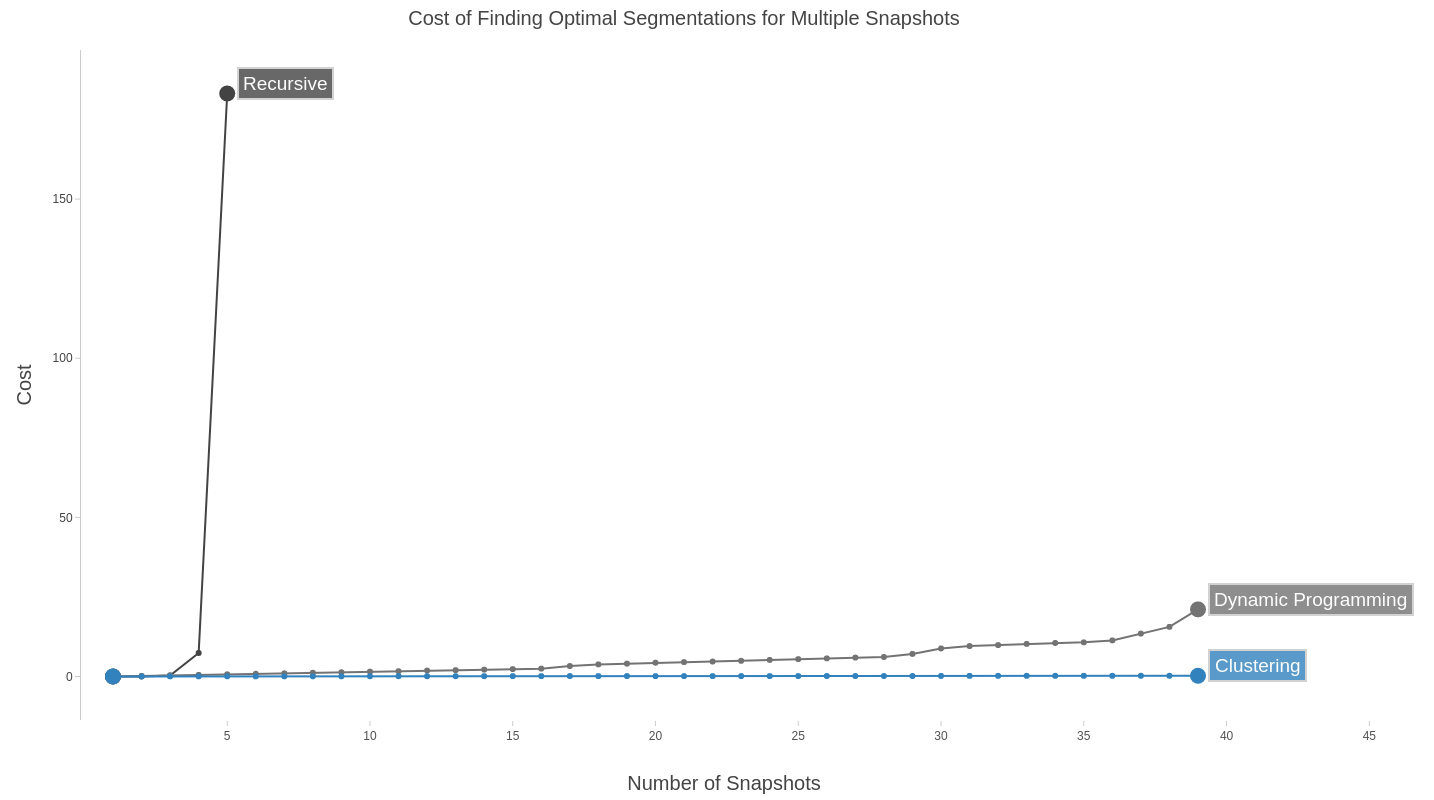
\includegraphics[width=\textwidth]{figs/variable_snapshots.jpg}
				\caption{Optimization time with respect to the number of snapshots}
				\label{fig:variable_snapshots}
			\end{figure} 

			\begin {center}
			\begin{table}
				\centering
				\caption{Optimization time with respect to the number of snapshots}
				\label {table:variable_snapshots}
				\begin{tabular}{p{2cm}p{3cm}p{3cm}p{3cm}}
					\hline
					Snapshots & Recursive      & Dynamic  & Clustering \\ \hline
					1 & 0.0002    & 0.01  & 0.01  \\  
					2 & 0.01    & 0.17  & 0.02  \\
					3 & 0.32    & 0.34  & 0.03  \\
					4 & 7.39 & 0.52  & 0.04  \\
					5 & 183.18 & 0.69  & 0.06 \\
					10 & N/A    & 1.52  & 0.08  \\
					15 & N/A & 2.33  & 0.12  \\ 
					20 & N/A & 4.33  & 0.12  \\ 
					25 & N/A & 5.46  & 0.14  \\ 
					30 & N/A & 8.81  & 0.17  \\
					35 & N/A & 10.74  & 0.21  \\
					40 & N/A & 21.09  & 0.24  \\\hline
				\end{tabular}
			\end{table}
			\end{center}

			Figure \ref{fig:variable_snapshots} and Table \ref{table:variable_snapshots} depict the observations of the experiment. The graph shows that in comparison with dynamic programming and K-means clustering, the recursive algorithm is computationally more expensive such that we couldnot utilize this technique to find more than 5 optimal timestamps for snapshots due to the large computational time. 

			\begin{figure}
				\centering
				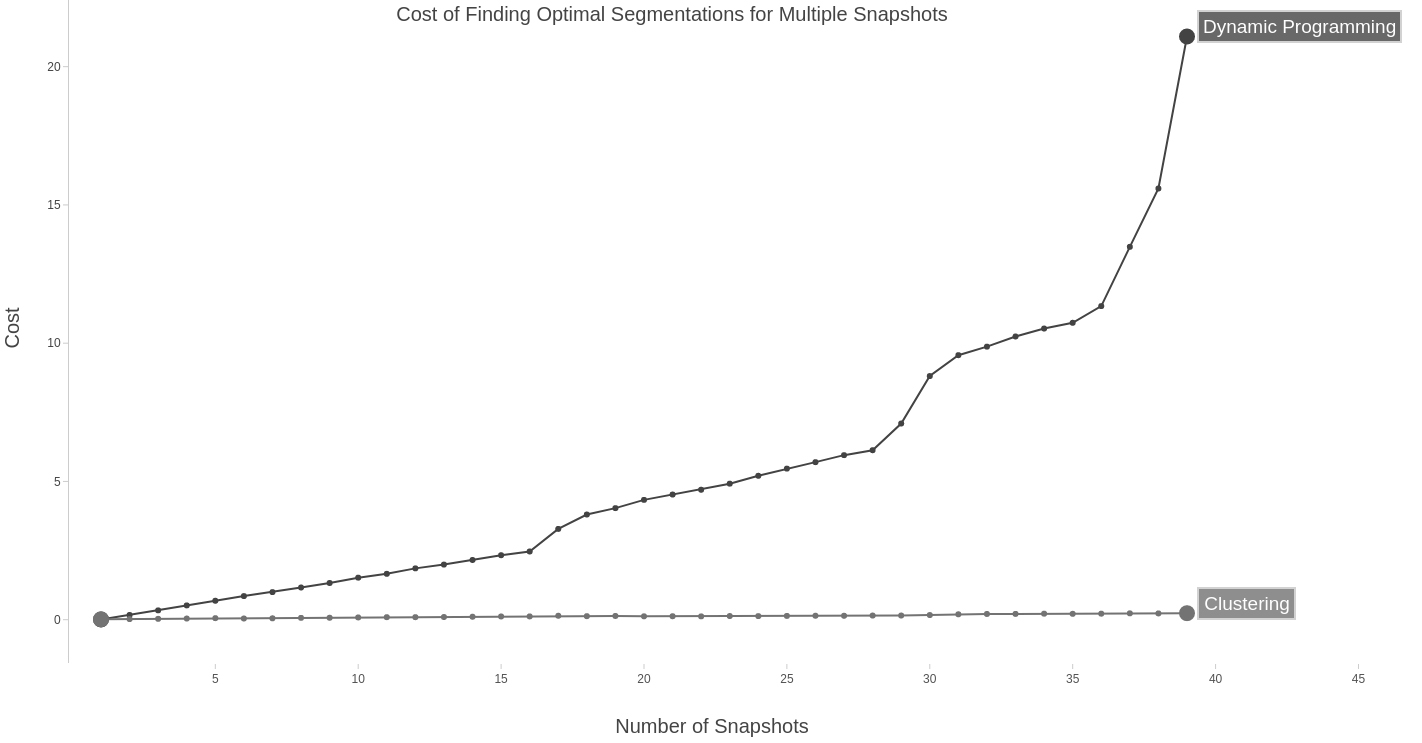
\includegraphics[width=\textwidth]{figs/multiSnapDouble.jpg}
				\caption{Optimization time with respect to the number of snapshots}
				\label{fig:variable_snapshots_2}
			\end{figure} 

			\begin{center}
			\begin{table}
				\centering
				\caption{Optimization time with respect to the number of snapshots}
				\label {table:variable_snapshots_2}
				\begin{tabular}{p{2cm}p{3cm}p{3cm}}
					\hline
					Snapshots  & Dynamic  & Clustering \\ \hline
					1 &   0.01 & 0.01 \\  
					2 &  0.17  & 0.02  \\
					3 &  0.34  & 0.03  \\
					4 & 0.52  & 0.04  \\
					5 &  0.69  & 0.06 \\
					10 &  1.52  & 0.08  \\
					15 & 2.33  & 0.12  \\ 
					20 & 4.33  & 0.12  \\ 
					25 & 5.46  & 0.14  \\ 
					30 & 8.81  & 0.17  \\
					35 & 10.74  & 0.21  \\
					40 & 21.09  & 0.24  \\\hline
				\end{tabular}
			\end{table}
			\end{center}
			Figure \ref{fig:variable_snapshots} and Table \ref{table:variable_snapshots_2}, have a closer look at the dynamic programming and clustering method of finding optimal timestamps. As it could be seen, the clustering method is computationally less expensive than the dynamic programming method.

			For the second experiment, we fixed the number of snapshots but made the number of queries variable. Our aim was to observe the performance of each approach as the number of queries grow. For this reason, we calculated 4 number of snapshots for queries ranging from 12 to approximately 180. 

			\begin{figure}
				\centering
				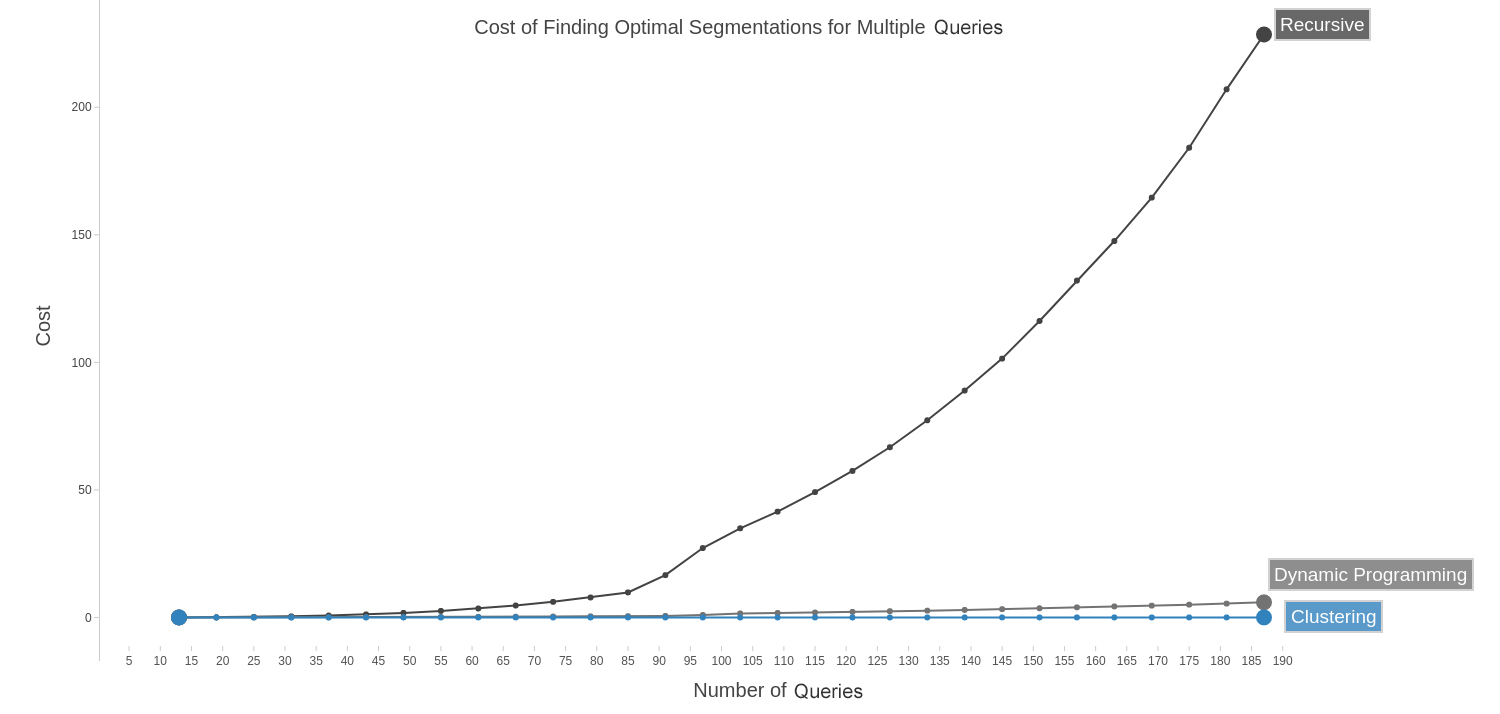
\includegraphics[width=\textwidth]{figs/multi_query.jpg}
				\caption{Optimization time with respect to the number of queries}
				\label{fig:variable_queries}
			\end{figure} 


			\begin {center}
			\begin{table}
				\centering
				\caption{Optimization time with respect to the number of queries}
				\label {table:variable_queries}
				\begin{tabular}{p{2cm}p{3cm}p{3cm}p{3cm}}
					\hline
					Queries & Recursive      & Dynamic  & Clustering \\ \hline
					13 & 0.05    & 0.01  & 0.02  \\  
					43 & 1.23    & 0.13  & 0.03  \\
					73 & 6.15    & 0.39  & 0.03  \\
					103 & 34.98 & 1.60  & 0.03  \\
					133 & 77.31 & 0.69  & 0.04 \\
					163 & 147.57 & 4.35  & 0.04  \\
					187 & 228.52 & 5.96  & 0.04  \\\hline
				\end{tabular}
			\end{table}
			\end{center}

			Figure \ref{fig:variable_queries_2} and Table \ref{table:variable_queries_2} shows that similar to the previous experiment, recursive algorithm has proven to be expensive in computing the optimal timestamps for the snapshots. To see the difference between the dynamic programming and the clustering method, we compared the performance of both in Figure \ref{} and Table \ref{}. These results also show that utilizing the clustering method is computationally more optimal than the other two method.

			\begin{figure}
				\centering
				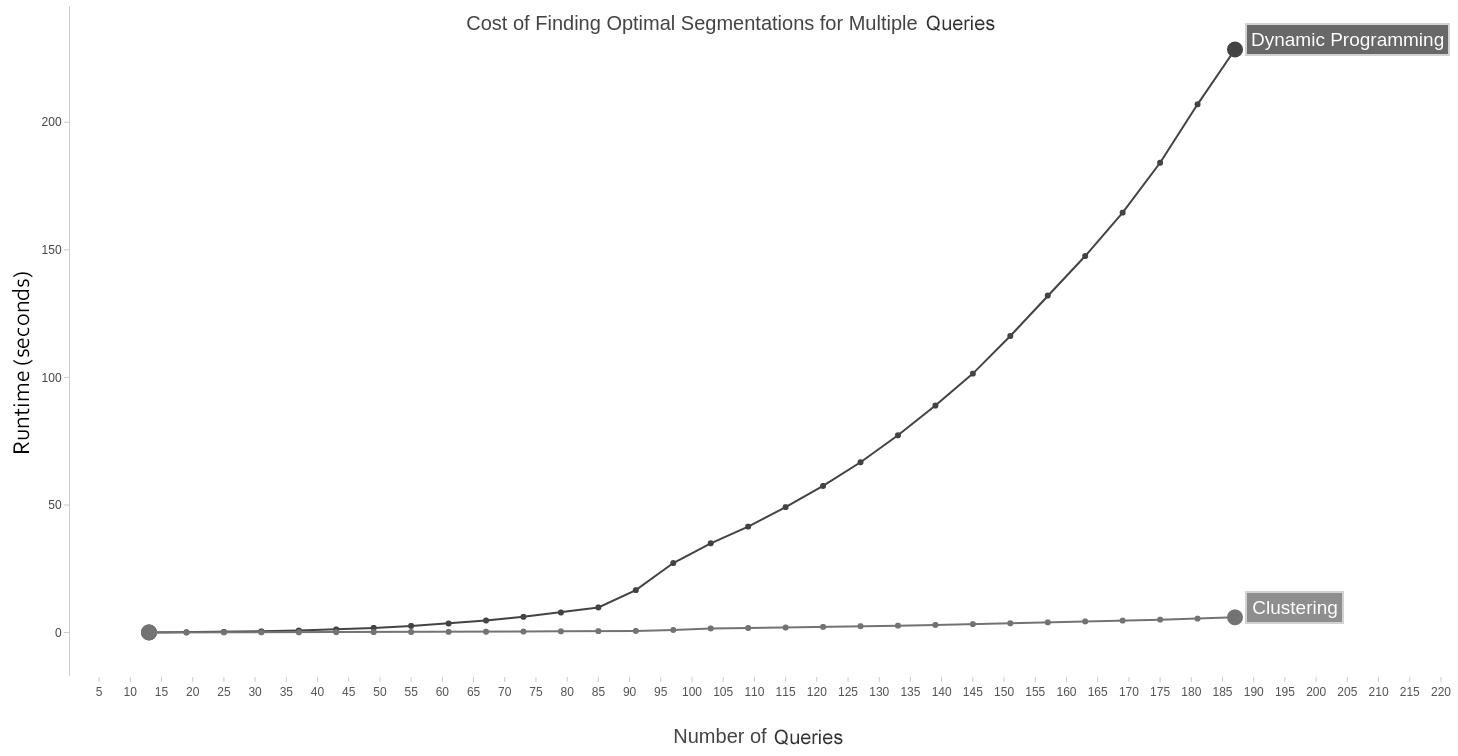
\includegraphics[width=\textwidth]{figs/multi_query_2.jpg}
				\caption{Optimization time with respect to the number of queries}
				\label{fig:variable_queries_2}
			\end{figure} 


			\begin {center}
			\begin{table}
				\centering
				\caption{Optimization time with respect to the number of queries}
				\label {table:variable_queries_2}
				\begin{tabular}{p{2cm}p{3cm}p{3cm}p{3cm}}
					\hline
					Queries  & Dynamic  & Clustering \\ \hline
					13 & 0.01  & 0.02  \\  
					43 & 0.13  & 0.03  \\
					73 & 0.39  & 0.03  \\
					103 & 1.60  & 0.03  \\
					133 & 0.69  & 0.04 \\
					163 & 4.35  & 0.04  \\
					187 & 5.96  & 0.04  \\\hline
				\end{tabular}
			\end{table}
			\end{center}

			\subsection{Evaluating the heuristic method} \label{sec:evaluating_heuristic}
			In the previous section we showed that the heuristic method (K-Means clustering method in this case) is computationally more favorable than the recursive algorithm and dynamic programming method. However unlike recursive algorithm and dynamic programming which compute the exact optimal timestamps for the snapshots, the heuristic method approximates the optimal timestamps. Because of this, in the heuristic method, finding the most optimal timestamps for the snapshots is not guaranteed. Therefore a comparison was needed to evaluate if the heuristic method could be chosen over the other two method.

			We previousely showed that as the number of snapshots grow, the overall cost of answering to the queries drops. In this experiment, we compared the outcome of the dynamic programming and K-Means clustering method in varying number of snapshots to see how increasing the number of snapshots affect the overall cost of query answering in both methods. As it could be seen in Figure \ref{fig:dynamic_vs_heuristic} and Table \ref{table:dynamic_vs_heuristic}, the outcome of dynamic programming and heuristic method is slightly different but the all in all the result of the heuristic method is satisfactory.

			\begin{figure}
				\centering
				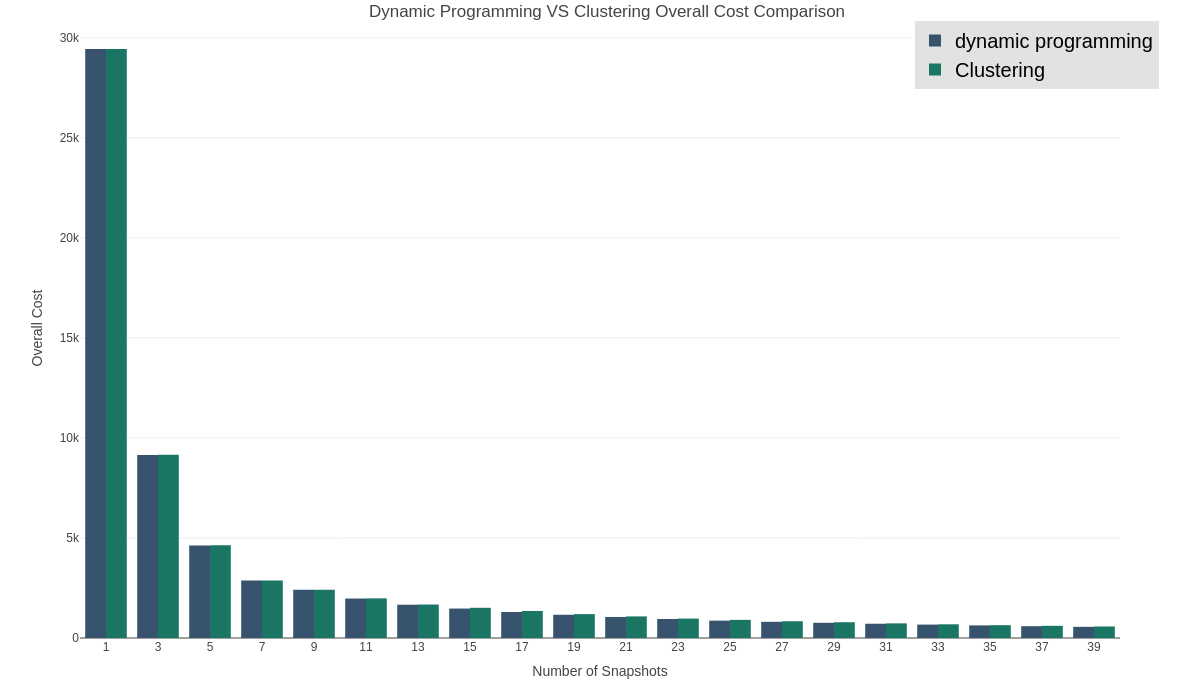
\includegraphics[width=\textwidth]{figs/dynamic_vs_clustering.jpg}
				\caption{Comparing the outcome of dynamic programming with the heuristic method}
				\label{fig:dynamic_vs_heuristic}
			\end{figure} 

			\begin {center}
			\begin{table}
				\centering
				\caption{Comparing the outcome of dynamic programming with the heuristic method}
				\label {table:dynamic_vs_heuristic}
				\begin{tabular}{p{2cm}p{3cm}p{3cm}p{3cm}}
					\hline
					Snapshots & Dynamic  & Clustering \\ \hline
					1 & 29439.26  & 29439.26  \\  
					3 & 9141.55  & 9159.13  \\
					5 & 4626.77  & 4630.08  \\
					7 & 2867.74  & 2867.74  \\
					9 & 2410.46  & 2412.62 \\
					11 & 1972.14  & 1980.95  \\
					13 & 1664.14  & 1673.32  \\
					15 & 1471.58  & 1509.57  \\
					17 & 1300.32  & 1351.44  \\
					19 & 1162.25  & 1194.61  \\
					21 & 1051.97  & 1079.71  \\
					23 & 951.06  & 970.72  \\
					25 & 867.35  & 907.30  \\
					27 & 810.01  & 836.97  \\
					29 & 759.69  & 787.86  \\
					31 & 713.04  & 731.61  \\
					33 & 670.39  & 684.13  \\
					35 & 629.69  & 640.58  \\
					37 & 591.08  & 608.96  \\
					39 & 557.81  & 575.97  \\\hline
				\end{tabular}
			\end{table}
			\end{center}

			The results of K-Means clustering method shown in Figure \ref{fig:dynamic_vs_heuristic} and Table \ref{table:dynamic_vs_heuristic} obtained by performing 300 number of iterations to find the appropriate centroids and clusters from the queries. Although 300 iterations improves the precision of the outcome but we were interested to see if we can lower the number of iterations for the sake of saving more time but still get satisfactory results. Therefore we lowered the number of iterations to 30 and compared the runtime with 300 iterations. Figure \ref{fig:clustering_comparison_multiQuery} shows the runtime comparison of K-Means clustering method with 300 iterations and 30 iterations for fixed number of queries but variable number of snapshots and Figure \ref{fig:clustering_comparison_multiSnap} shows the same comparison for fixed number of snapshots but varying number of queries.

			\begin{figure}
				\centering
				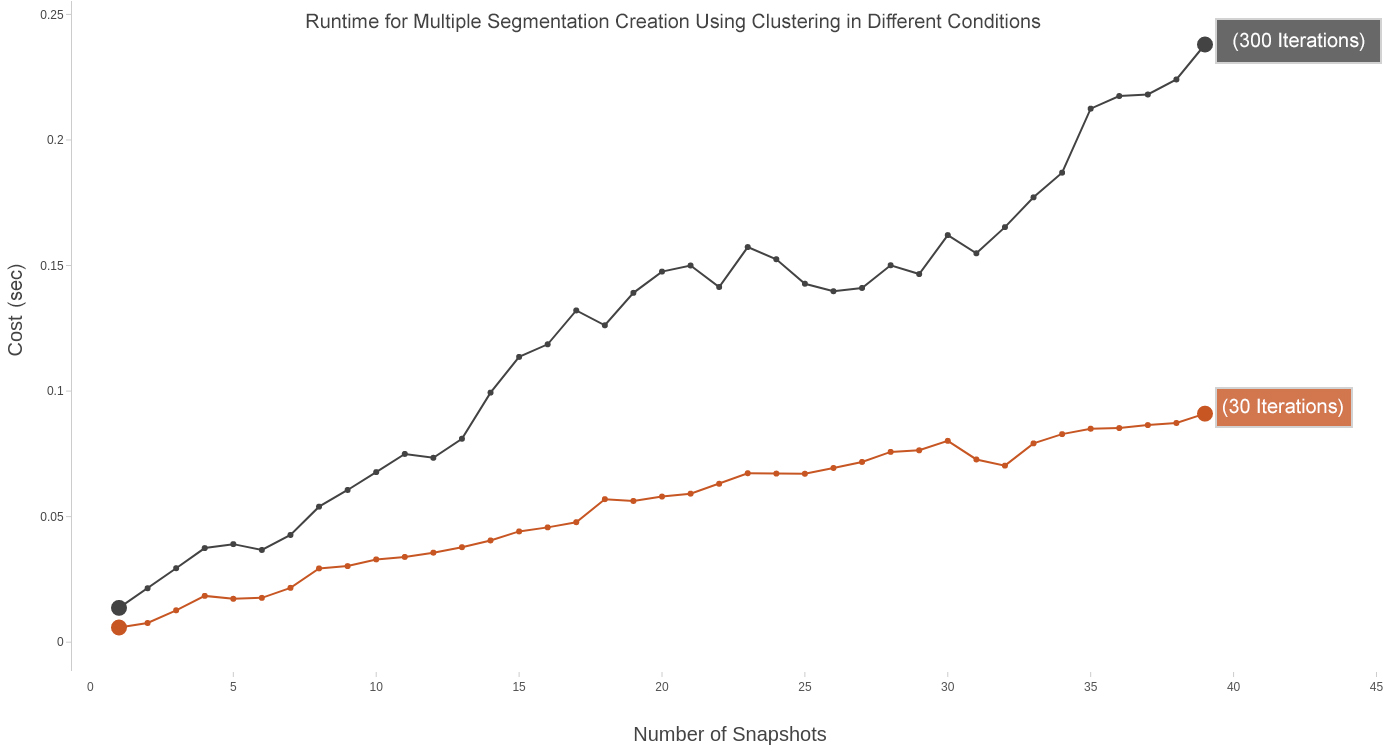
\includegraphics[width=\textwidth]{figs/multiSnap_clustering.jpg}
				\caption{Comparing the runtime of K-Means clustering method with 30 and 300 iterations for variable number of snapshots}
				\label{fig:clustering_comparison_multiSnap}
			\end{figure} 

			\begin{figure}
				\centering
				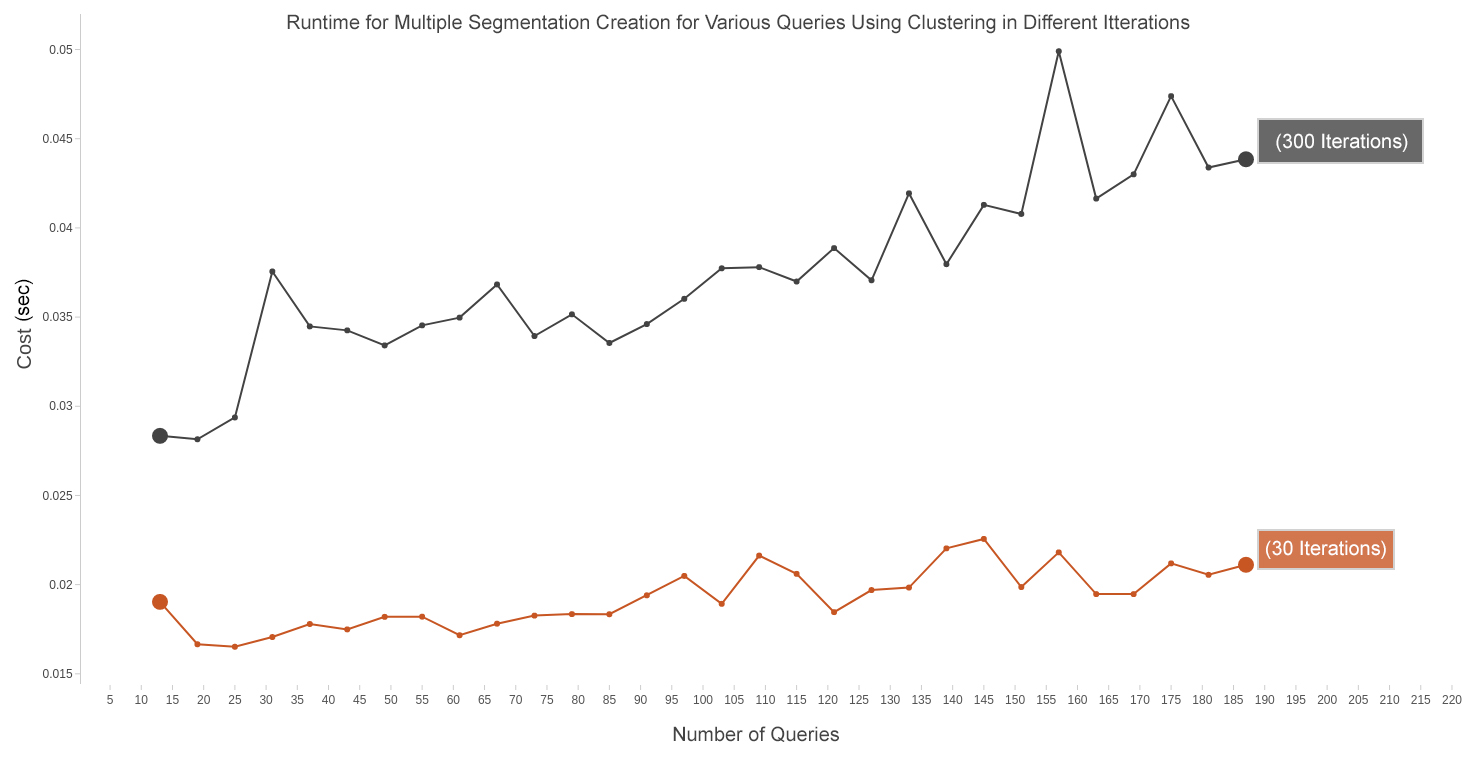
\includegraphics[width=\textwidth]{figs/multiQuery_clustering.jpg}
				\caption{Comparing the runtime of K-Means clustering method with 30 and 300 iterations for variable number of queries}
				\label{fig:clustering_comparison_multiQuery}
			\end{figure} 

			We further lowered the number of iterations to 5 and compared the overal cost of query answering in variable number of snapshots. As seen in Figure \ref{fig:compare_clusterings_iterations} and Table \ref{table:compare_clustring_iterations}, the cost of query answering is more expensive when 5 iterations were used in K-Means clustering however this difference is not significant as the number of snapshots grow.

			\begin{figure}
				\centering
				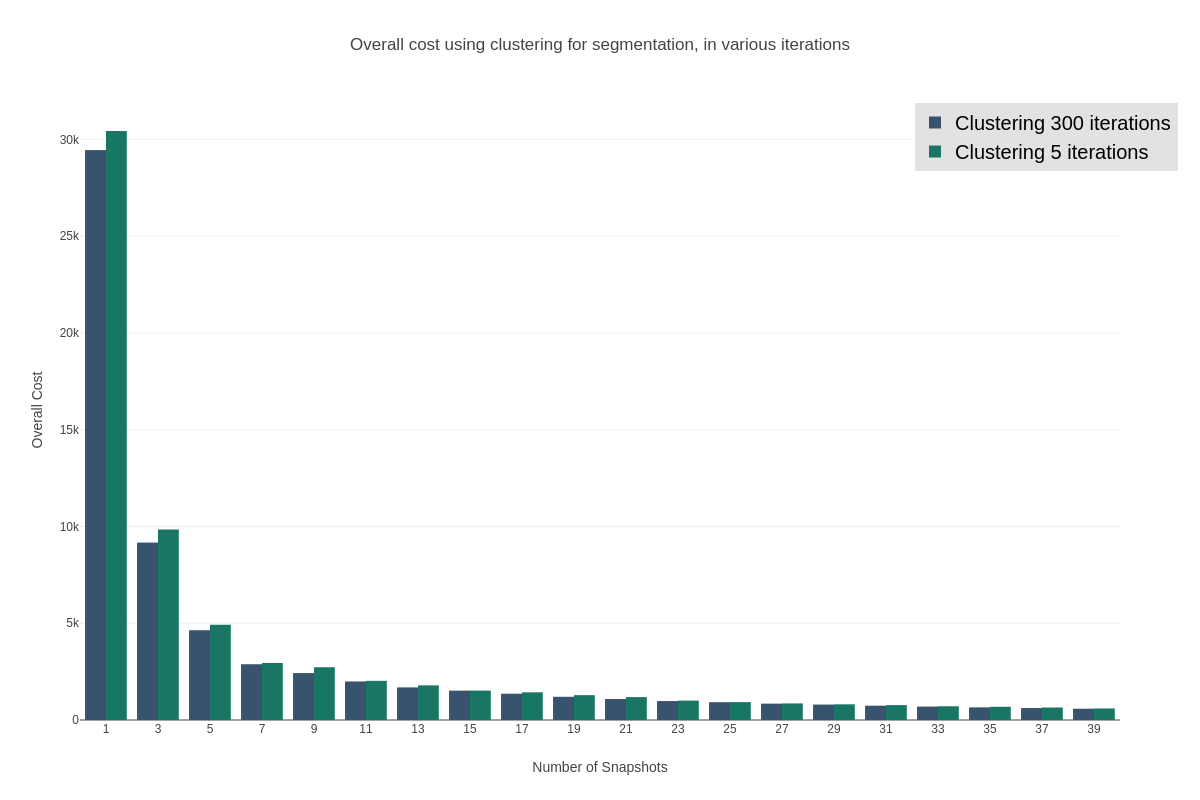
\includegraphics[width=\textwidth]{figs/compare_clustering_iterations.png}
				\caption{Comparing the overal cost of query answering in variable number of snapshots using K-Means clustering method with 30 and 300 iterations to find optimal timestamps for snapshots}
				\label{fig:compare_clusterings_iterations}
			\end{figure} 

			\begin {center}
			\begin{table}
				\centering
				\caption{Comparing the overal cost of query answering in variable number of snapshots using K-Means clustering method with 30 and 300 iterations to find optimal timestamps for snapshots}
				\label {table:compare_clustring_iterations}
				\begin{tabular}{p{2cm}p{3cm}p{3cm}p{3cm}}
					\hline
					Snapshots  & 300 iterations  & 5 iterations \\ \hline
					1 & 29439.26 & 30439.26 \\  
					3 & 9159.13  & 9841.13\\
					5 & 4630.08  & 4921.08\\
					7 & 2867.74  & 2945.76\\
					9 & 2412.62  & 2732.38\\
					11 & 1980.95  & 2023.24\\
					13 & 1673.32  & 1789.50\\
					15 & 1509.57  & 1521.68\\
					17 & 1351.44  & 1430.66\\
					19 & 1194.61  & 1284.61\\
					21 & 1079.71  & 1182.71\\
					23 & 970.72  & 1002.57\\
					25 & 907.30  & 923.30\\
					27 & 836.97  & 856.83\\
					29 & 787.86  & 811.08\\
					31 & 731.61  & 769.83\\
					33 & 684.13  & 710.49\\
					35 & 640.58  & 683.60\\
					37 & 608.96  & 645.74\\
					39 & 575.97  & 595.89\\\hline
				\end{tabular}
			\end{table}
			\end{center}

		\section{Discussion}
				Each method has their pros and cons which are shown in Table \ref{table:segmentation_comparison}. In the next section we support the comparison between methods with different experiments and we depict the observations followed by drawing a conclusion. 
		
		\begin{center}
			\begin{table}
				\centering
				\small
				\caption{Snapshot $s_2$ at $t = 2018-03-15$}
				\label{table:segmentation_comparison}
				\begin{tabular}{p{4cm}p{4cm}p{4cm}}
					\hline
					method & Pros  & Cons  \\ \hline
					Recursive algorithm & Exact optimal solution & computationally expensive for large number of queries and segmentations   \\ \hline
					Dynamic programming & Exact optimal solution & computationally expensive for large number of queries and segmentations\\ 
					  & Computationally cheaper than dynamic programming &    \\ \hline
					K-Means clustering & Fast in computation & optimal solution not guaranteed \\ \hline
				\end{tabular}
			\end{table}
		\end{center}